\minpurp{Architekturmuster}
Vorraussetzung: Modularität

\minmeth{Model-View-Controller}
Darstellung von variablen Daten in verschiedenen Sichten

Leichte Änderbarkeit der Views => Unabhängig vom Kern implementiert;

Direke Anpassung der Sichten bei Änderungen

\submeth{Lösung}
Modularisierung:

Model: Kernfunktionalität und Datenmodell; registriert und informiert View u. Controller

View: Darstellung der vom Model abgefragten Daten

Controller: Auswertung Benutzereingaben => Aufruf von Model bzw. Viewfunktionen

Bei Implementierung als Observer Pattern: Observable->Model, Observer->View,Controller

\minpurp{Design Pattern}
Vorraussetzung: Objektorientierung

\minmeth{Strategy} Austauschbare Algorithmen\\
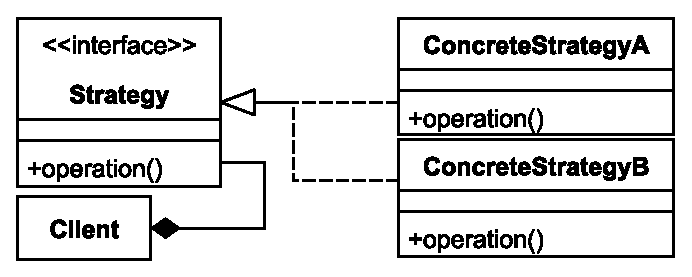
\includegraphics[width=0.2\textwidth]{strategy}

\minmeth{Observer} Informieren von Objekten über Zustandsänderungen eines Objektes\\
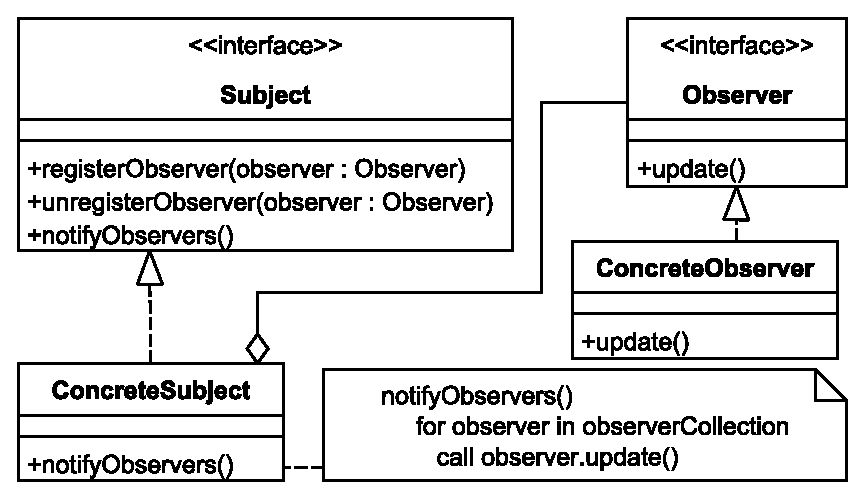
\includegraphics[width=0.24\textwidth]{observer}
Varianten:\\
Pull: keine information im notify
Push: Zustandsänderung wird mitgeschickt

\minmeth{Iterator} Sequentieller Zugriff auf Elemente eines Aggregats ohne interna preiszugeben. 
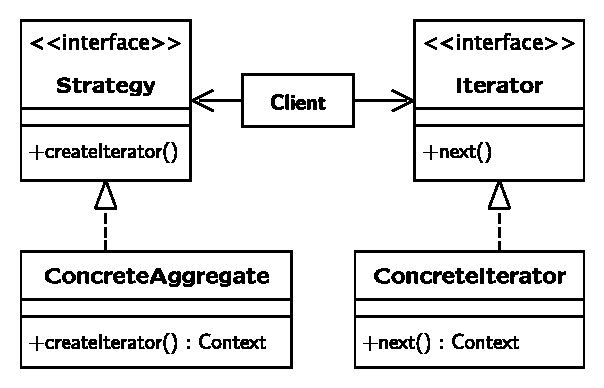
\includegraphics[width=0.3\textwidth]{iterator}

\minmeth{Composite} Abbildung einer Hierarchie, Verwendung der Teile unabhängig von der Position (Knoten vs Blatt)\\
Lösung: Schnittstelle mit Operationen für Hierarchieverwaltung und Elementfunktionen => Keine Unterschiede für Client
\includegraphics[width=0.2\textwidth]{Composite}

\minmeth{Factory Method}

Problem: Objekt erzeugen. Nur Schnittstelle nicht konkrete Klasse bekannt. 

Factory Method: Hook für Subklasse, um Verhalten in der Basisklasse zu konfigurieren. Product und Creator bilden häufig „parallele“ Klassenhierarchien.
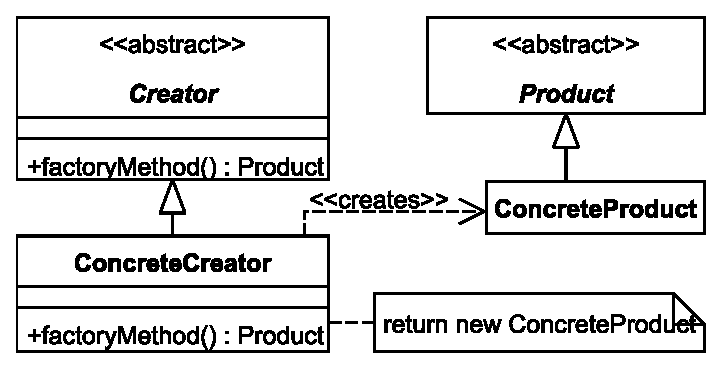
\includegraphics[width=0.3\textwidth]{factory}

\minmeth{Abstract Factory}

entkopplung Objekterzeugung/-verwendung. Factory Method legt Klasse der Objekte fest. 

Delegieren Objekterzeugung.

Factory Instanzen implementieren Factory Methoden für Objekte einer Klassenfamilie

Schnittstelle AbstractFactory sieht eine Factory Methode je
Produkt vor. Definiere pro Produktfamilie eine ConcreteFactory Klasse

=> System arbeitet unabhängig von Objekterzeugung. Austausch
von Produktfamilien ist einfach. Schwierig, neue Produkte einzuführen, da alle
Factoryklassen um eine Methode ergänzt werden müssen.

\includegraphics[width=0.3\textwidth]{abstractfactory-eps-converted-to}

\minpurp{Programmieridiome}
Vorraussetzung: Konkrete Sprache

\minmeth{Mixin} Erweitert bestehende Klasse ohne Vererbung zu verändern\\
\textcolor{mehrblau}{ohne Mehrfachvererbung}, \textcolor{mehrred}{mit Mehrfachvererbung}\\
\includegraphics[width=0.24\textwidth]{mixinjava}
